\section{Event Selection Summary}

The anlaysis have different layers of selection here we will summarize all the selection requriements mentioned in the previous chapter with the accociated efficiencies for each selection layer. The starting selection layer which we will call as preselection has the following requirements:

\begin{itemize}
\item Medium working point id/isolated \et$^{\gamma} > 45 \GeV $
\item $|\eta^{\gamma}| < 1.442$
\item $\sigma_{i{\eta}i{\eta}} > 0.001$ , $\sigma_{i{\phi}i{\phi}} > 0.001$ , swiss cross $> 0.9$ , $ 1.0 > R_{9} > 0.9$
%\item \met Noise Cleaning Filters
\item \met$ > 40 $
\end{itemize}

Photon id working point, along with energy and cut on the MT has been studied extensively. The cuts have been chosen to maximize the S/$\sqrt(S+B)$. And the different working points tried can be seen in Fig~\ref{fig:optimize}. We have further optimized the cut on Met Significance using all the cuts but the cut on Met Significance. This means, that we have implement the MHT Minimization cuts, and then scanned different working points for Met Significance. The cut value has been optimized with respect to the expected limits. The plot showing the working point can be seen in Fig~\ref{fig:optimize}.

\begin{figure}[htb]
  \begin{center}
    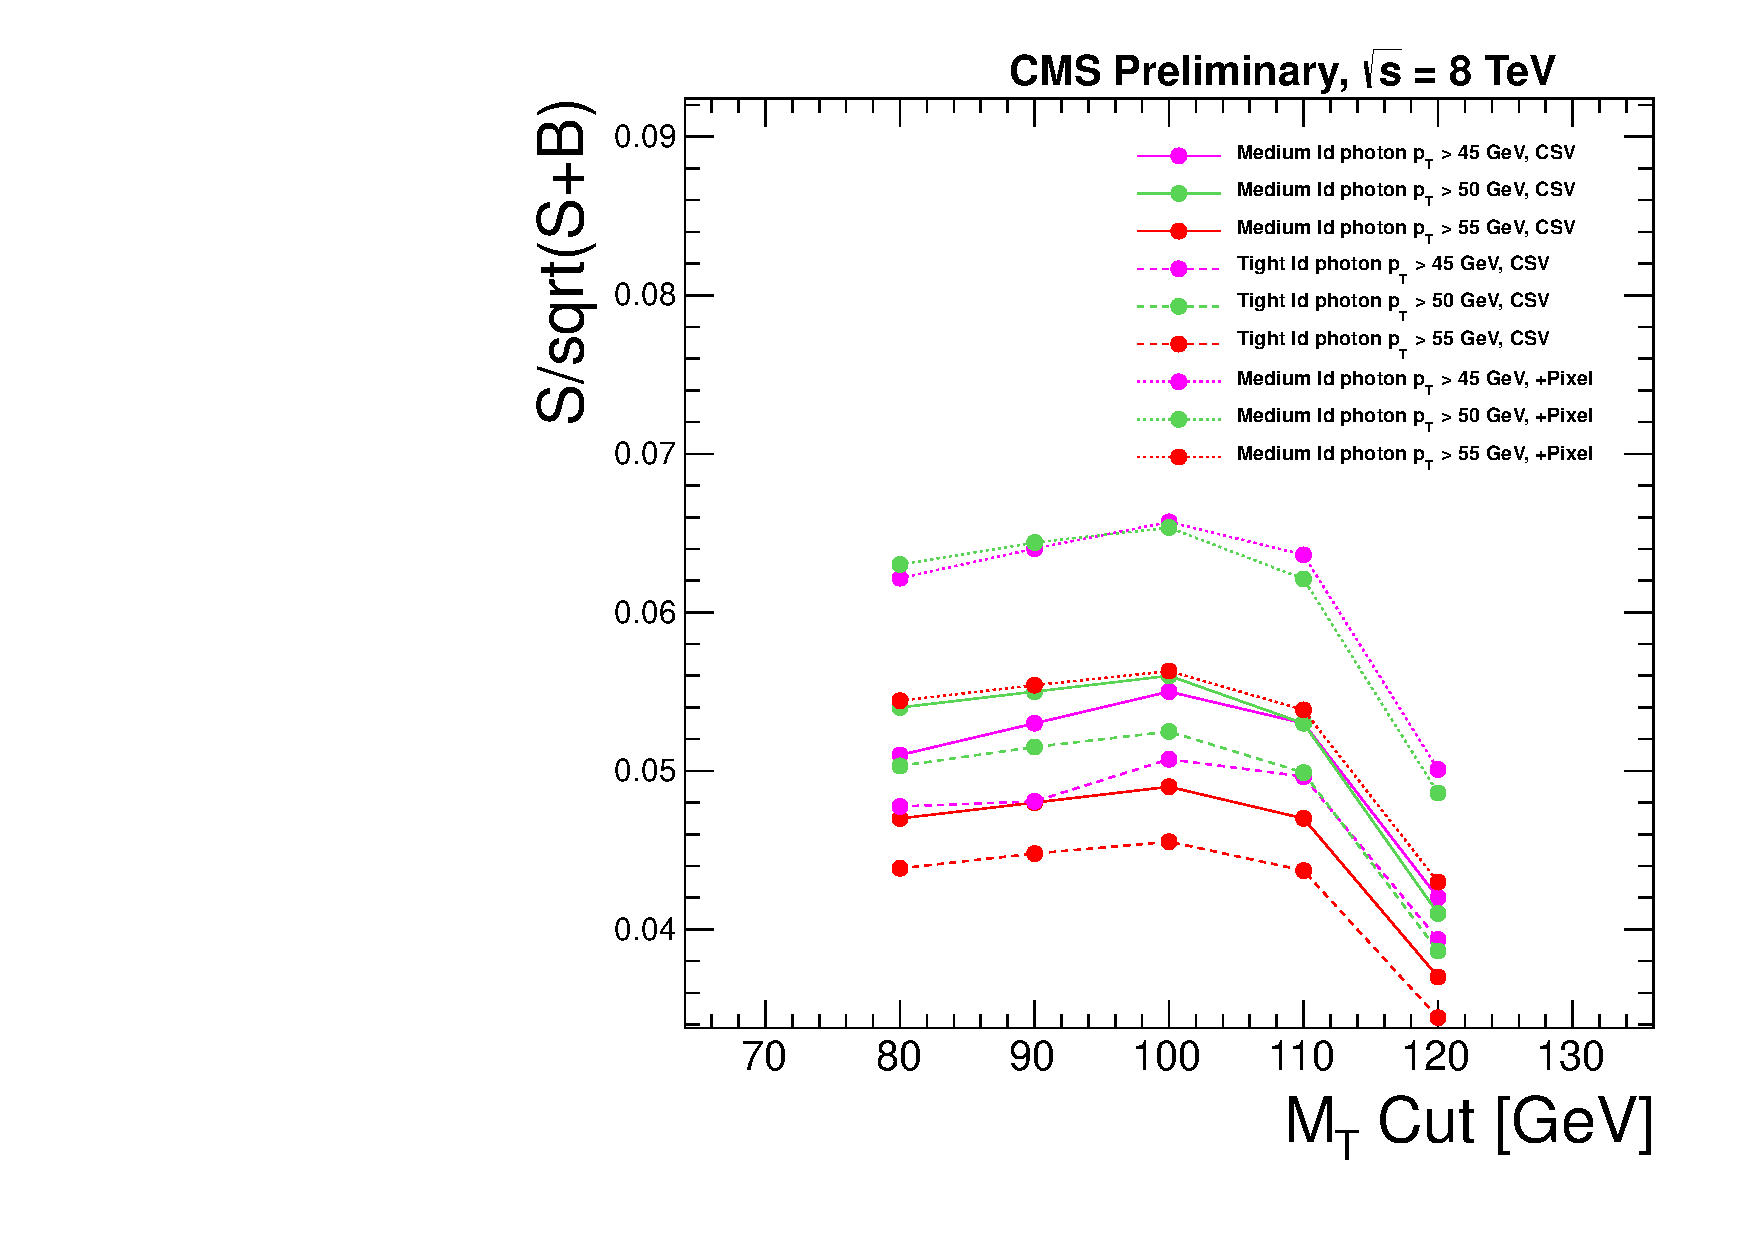
\includegraphics[width=0.48\textwidth,angle=0]{analysis_figs/photon_optimize}\hfill
     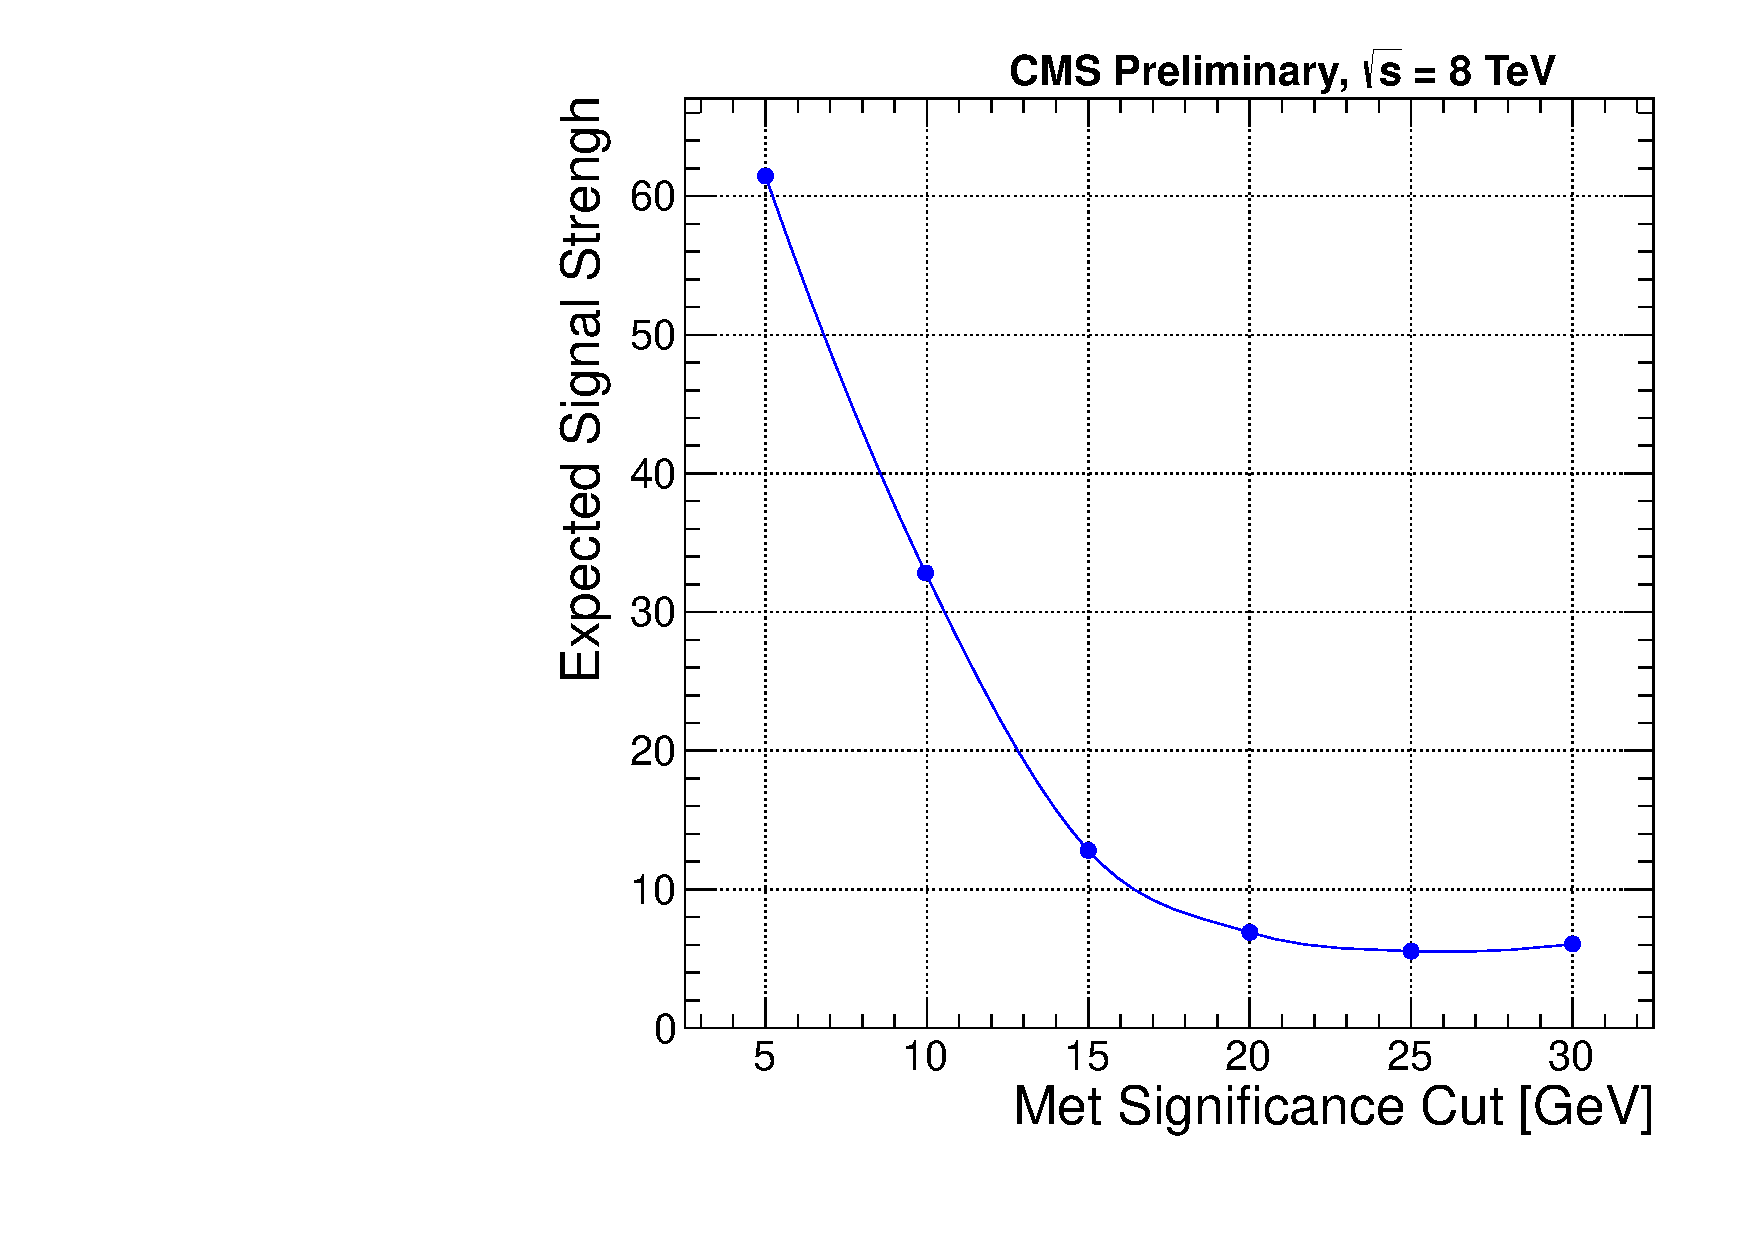
\includegraphics[width=0.48\textwidth,angle=0]{analysis_figs/metsig_optimize.pdf}\hfill
    \caption{The optimization plots on photon energy working point, MT and Met Significance.}
  \end{center}
  \label{fig:optimize}
\end{figure}

The following selection is required depending on the model dependent and model independent results.

\begin{table}[!h]
\center
{
\begin{tabular}{|c|c|c|c|c|c|c|}
\hline
Selection &  $\gamma +$ jets & ${\rm jet}\rightarrow \gamma$ & ${\rm e} \rightarrow \gamma$ & $Z( \to \nu \bar{\nu} )+\gamma$ & $W(\to \ell\nu)+\gamma $ & Other \\
\hline
Lepton Veto   &  99.80 $\%$ & 99.54 $\%$ & 95.77 $\%$ & 99.96 $\%$ & 61.68 $\%$ & 58.15 $\%$\\
N Jets$ < 2$  & 72.90 $\%$ & 76.76 $\%$ & 78.31 $\%$ & 90.87 $\%$ & 44.18 $\%$ & 51.62 $\%$ \\
$\Delta\Phi(\gamma,jet) < 2.5$ &  30.87 $\%$ & 26.22 $\%$ & 57.85 $\%$ & 83.40 $\%$ & 32.55 $\%$ & 38.63 $\%$\\
\hline
\end{tabular}
\caption{The cumulative efficiencies of all the cuts at the model independent selection layer}
\label{table:modelindep_eff}
}

\end{table}

\begin{table}[!h]
\center
{
\begin{tabular}{|c|c|c|c|c|c|c|c|}
\hline
Selection & $M_\chi = 70 \GeV$ & $\gamma +$ jets & ${\rm jet}\rightarrow \gamma$ & ${\rm e} \rightarrow \gamma$ & $Z( \to \nu \bar{\nu} )+\gamma$ & $W(\to \ell\nu)+\gamma $ & Other \\
\hline
Lepton Veto & 99.94 $\%$ & 99.80 $\%$ & 99.54 $\%$ & 95.77 $\%$ &  99.96 $\%$ &  61.68  $\%$ &  58.15 $\%$\\
$M_{T} > 100$ & 61.60 $\%$ & 29.13 $\%$ & 22.39 $\%$ & 34.22 $\%$ & 86.70 $\%$ & 33.81 $\%$ & 29.93 $\%$  \\
$H_{T} < 100$ & 59.44 $\%$ & 18.80 $\%$ & 16.75 $\%$ & 29.70 $\%$ & 78.44 $\%$ & 25.81 $\%$ & 28.35 $\%$  \\
$\tilde{\met} > 45 $ & 53.97 $\%$ & 7.12 $\%$ & 4.35 $\%$ & 22.19 $\%$ & 76.06 $\%$ & 22.44 $\%$ & 25.32 $\%$  \\
$P(\chi^2) < 10^{-3}$ & 30.48 $\%$ & 3.25 $\%$ & 1.87 $\%$ & 11.10 $\%$ & 62.58 $\%$ & 15.94 $\%$ & 16.52 $\%$  \\
Met Sig. $> 20 $ & 13.17 $\%$ & 0.07 $\%$ & 0.28 $\%$ & 4.40 $\%$ & 43.96 $\%$ & 9.47 $\%$ & 8.99 $\%$  \\
Angle $ > 1.2$  & 11.13 $\%$ & 0.07 $\%$ & 0.18 $\%$ & 4.08 $\%$ & 38.94 $\%$ & 8.24 $\%$ & 8.23 $\%$  \\
\et$^{\gamma} < 60 \GeV $ & 8.24 $\%$ & 0.02 $\%$ & 0.08 $\%$ & 1.99 $\%$ & 7.41 $\%$ & 2.25 $\%$ & 1.94 $\%$ \\
\hline
\end{tabular}
\caption{The cumulative efficiencies of all the cuts at the model dependent selection layer}
\label{table:modeldep_eff}}

\end{table}
